% formal/stateless.tex
% SPDX-License-Identifier: CC-BY-SA-3.0

\section{Stateless Model Checkers}
\label{sec:formal:Stateless Model Checkers}

앞의 섹션에서 설명한 SAT-solver 방법은 상당히 편리하고 강력합니다만, 모든
가능한 수행 경우를 상태를 포함해서 모두 추적하는건 상당한 오버헤드를 일으킬 수
있습니다.
실제로, 메모리와 CPU-time 오버헤드는 적당하게 검증될 수 있는 프로그램의 크기를
제한하게 되는데, 이는 덜 정확한 방법들이 더 커다란 프로그램의 버그를 찾아낼 수
있을까 하는 질문을 품게 합니다.

이 질문에 대한 판정단은 아직 없지만, Nidhugg~\cite{CarlLeonardsson2014Nidhugg}
같은 stateless model checker 들은 일부 경우에 더 큰 프로그램들을
처리했습니다~\cite{SMC-TreeRCU}.
또한, Nidhugg 는 일부 리눇 크너러 RCU 검증 시나리오에서 \co{cbmc} 보다 열배
넘게 빨랐습니다.
물론, Nidhugg 의 속도와 확장성의 장점은 데이터 비결정성을 처리하지 않는다는
사실과 연관되어 있습니다만, 이는 이 특정 검증 시나리오에서는 문제가 되지
않았습니다.
\iffalse

The SAT-solver approaches described in the previous section are quite
convenient and powerful, but the full tracking of all possible
executions, including state, can incur substantial overhead.
In fact, the memory and CPU-time overheads can sharply limit the size
of programs that can be feasibly verified, which raises the question
of whether less-exact approaches might find bugs in larger programs.

\begin{figure}[tbp]
\centering
\resizebox{2.1in}{!}{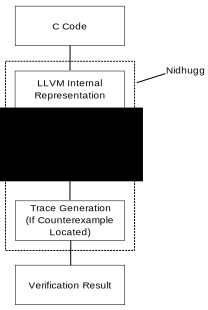
\includegraphics{formal/nidhugg}}
\caption{Nidhugg Processing Flow}
\label{fig:formal:Nidhugg Processing Flow}
\end{figure}

Although the jury is still out on this question, stateless model
checkers such as Nidhugg~\cite{CarlLeonardsson2014Nidhugg} have in
some cases handled larger programs~\cite{SMC-TreeRCU}, and with
similar ease of use, as illustrated by
Figure~\ref{fig:formal:Nidhugg Processing Flow}.
In addition, Nidhugg was more than an order of magnitude faster than
was \co{cbmc} for some Linux-kernel RCU verification scenarios.
Of course, Nidhugg's speed and scalability advantages are tied to
the fact that it does not handle data non-determinism, but this
was not a factor in these particular verification scenarios.
\fi

그러나, \co{cbmc} 에서와 같이, Nidhugg 는 아직 리눅스 커널 RCU 의 메인테이너가
알지 못한 버그를 찾지는 못했습니다.
하지만, 리눅스 커널 RCU 의 역사상의 버그가 메인테이너가 생각했던 것과 다른
커밋으로 수정되었음을 보일 수는 있었으며, 이는 Nidhugg 와 같은 stateless model
checker 들이 언젠가는 병렬 코드의 동시성 버그를 찾는데 유용해지는 날이 올
것이란 희망을 품게 합니다.
\iffalse

Nevertheless, as with \co{cbmc}, Nidhugg has not yet been able to
locate a bug that Linux-kernel RCU's maintainer was not already
aware of.
However, it was able to demonstrate that one historical bug in
Linux-kernel RCU was fixed by a different commit than the maintainer
thought, which gives some additional hope that stateless model checkers
like Nidhugg might someday be useful for finding concurrency bugs in
parallel code.
\fi
